\section{tasks::subtract\-Dark Class Reference}
\label{classtasks_1_1subtractDark}\index{tasks::subtractDark@{tasks::subtractDark}}
Inheritance diagram for tasks::subtract\-Dark::\begin{figure}[H]
\begin{center}
\leavevmode
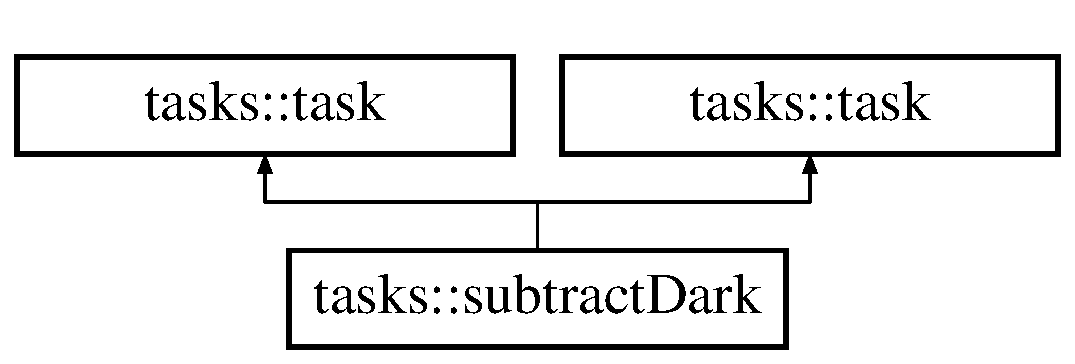
\includegraphics[height=2cm]{classtasks_1_1subtractDark}
\end{center}
\end{figure}
\subsection*{Public Member Functions}
\begin{CompactItemize}
\item 
def \textbf{run}\label{classtasks_1_1subtractDark_ee00c9be02dbec33b836e9e598ae215f}

\item 
def \textbf{run}\label{classtasks_1_1subtractDark_ee00c9be02dbec33b836e9e598ae215f}

\end{CompactItemize}
\subsection*{Static Public Attributes}
\begin{CompactItemize}
\item 
string \textbf{name} = '{\bfsubtract\-Dark}'\label{classtasks_1_1subtractDark_7f8d364c1eb69c54a85896fdf5371ff5}

\item 
string \textbf{button\-Text} = 'Subtrac dark '\label{classtasks_1_1subtractDark_dc63151f70d115268d7b0fdf43fa018f}

\end{CompactItemize}


\subsection{Detailed Description}


\footnotesize\begin{verbatim}Subtract dark from an image using a master dark
\end{verbatim}
\normalsize
 



The documentation for this class was generated from the following files:\begin{CompactItemize}
\item 
old/PANICtool-1.0/tasks.py\item 
old/tasks.py\end{CompactItemize}
